
The C++ Standard Library provides a selection of random number distribution generators, each with its own properties. In this recipe, we examine a function to compare the different options by creating a histogram of their output.

\subsubsection{How to do it…}

Like the random number engines, the distribution generators have some common interface elements. Unlike the random number engines, the distribution generators have a variety of properties to set. We can create a template function to print a histogram of the various distributions, but the initializations of the various distribution generators vary significantly:

\begin{itemize}
\item 
We start with some constants:

\begin{lstlisting}[style=styleCXX]
constexpr size_t n_samples{ 10 * 1000 };
constexpr size_t n_max{ 50 };
\end{lstlisting}

The n\_samples constant is the number of samples to generate for each histogram – in this case, 10,000.

The n\_max constant is used as a divisor while generating our histograms.

\item 
Our histogram function takes a distribution generator as an argument and prints a histogram for that distribution algorithm:

\begin{lstlisting}[style=styleCXX]
void dist_histogram(auto distro,
		const string_view& dist_name) {
	std::default_random_engine rng{};
	map<long, size_t> m;
	
	// create the histogram map
	for(size_t i{}; i < n_samples; ++i)
		++m[(long)distro(rng)];
	
	// print the histogram
	auto max_elm_it = max_element(m.begin(), m.end(),
		[](const auto& a, const auto& b)
		{ return a.second < b.second; }
		);
	size_t max_elm = max_elm_it->second;
	size_t max_div = std::max(max_elm / n_max,
		size_t(1));
	cout << format("{}:\n", dist_name);
	for (const auto [randval, count] : m) {
		if (count < max_elm / n_max) continue;
		cout << format("{:3}:{:*<{}}\n",
			randval, ' ', count / max_div);
	}
}
\end{lstlisting}

The dist\_histogram() function uses a map to store the histogram. It then displays the histogram as a series of asterisks on the console.

\item 
We call dist\_histogram() from main(), like this:

\begin{lstlisting}[style=styleCXX]
int main() {
	dist_histogram(std::uniform_int_distribution<int>
		{0, 9}, uniform_int_distribution");
	dist_histogram(std::normal_distribution<double>
		{0.0, 2.0}, "normal_distribution");
	...
\end{lstlisting}

Calling the dist\_histogram() function is more complex than it was for the random number generators. Each random distribution class has a different set of parameters, according to its algorithm.

For the full list, refer to the distribution.cpp file in the GitHub archive.

Output:

\begin{center}
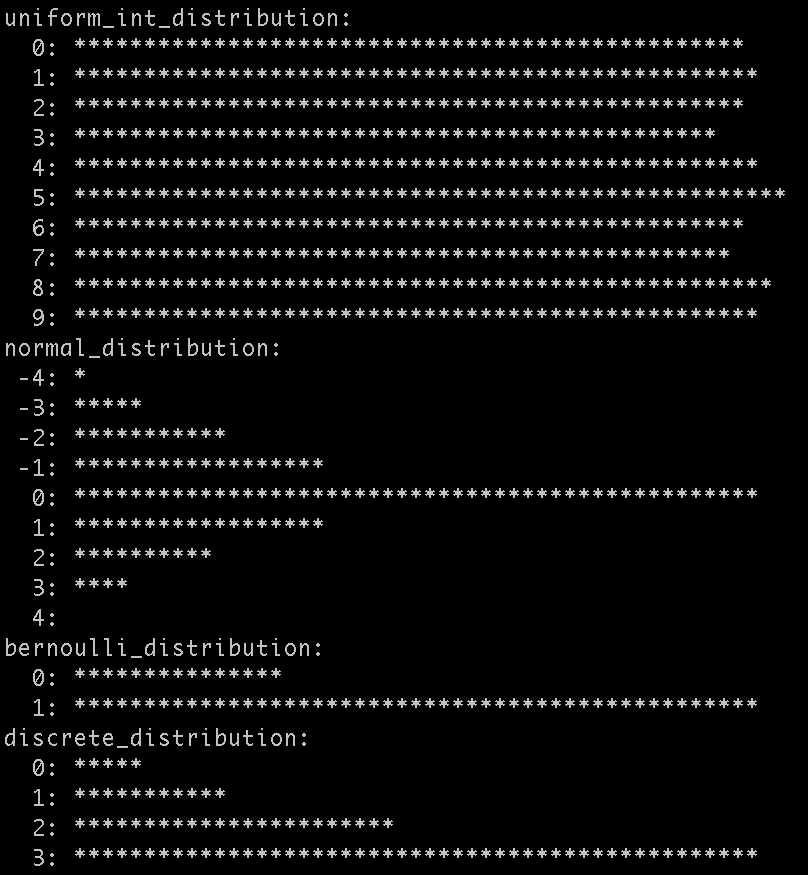
\includegraphics[width=0.8\textwidth]{content/chapter8/images/3.png}\\
Figure 8.3 – A screenshot of random distribution histograms
\end{center}

Each of the distribution algorithms produces very different output. You will want to experiment with the different options for each random distribution generator.

\end{itemize}

\subsubsection{How it works…}

Each of the distribution generators has a functor that returns the next value in the random distribution:

\begin{lstlisting}[style=styleCXX]
result_type operator()( Generator& g );
\end{lstlisting}

The functor takes a random number generator (RNG) object as an argument:

\begin{lstlisting}[style=styleCXX]
std::default_random_engine rng{};
map<long, size_t> m;
for (size_t i{}; i < n_samples; ++i) ++m[(long)distro(rng)];
\end{lstlisting}

For our purposes, we're using the std::default\_random\_engine for our RNG.

As with the RNG histogram, this is a useful tool to visualize the various random distribution algorithms available in the random library. You will want to experiment with the various parameters available for each algorithm.











